%\documentstyle[aas2pp4,epsf]{article}
%%%\documentstyle[aaspp4,epsf]{article}
%\documentstyle[12pt,aasms]{article}    % this is for a preprint
%(single-spaced)
%\documentstyle[aaspp4,epsf]{article} % this is for small print
%\documentstyle[12pt, aaspp4]{article}

%\documentstyle[11pt,aaspp]{article}
%\documentclass[12pt, preprint]{aastex} 

\documentclass[manuscript]{aastex}
%\documentclass[apj]{emulateapj}

%\documentclass[12pt, preprint,numberedappendix]{emulateapj}
%\documentstyle[12pt,aasms]{article}    % this is for submittal
                                       % (double-spaced)

%\documentstyle[12pt,aasms]{article}   \usepackage{emulateapj5} 

\usepackage{graphicx} 
\usepackage{amsmath}
\usepackage{hyperref}
\usepackage{amsfonts}
\usepackage{amsmath}
\usepackage{amssymb}
\usepackage{amsthm}
\usepackage{subeqnarray}
\usepackage{ulem}
%\bibliographystyle{apj}

\newcommand{\delad}{\nabla_{\rm ad}}
\newcommand{\delrad}{\nabla_{\rm rad}}
\newcommand{\emgr}[1]{\emph{ \color{gray} #1}}

\newcommand{\ie}{i.e.\ }
\newcommand{\eg}{e.g.\ }
\newcommand{\p}{\partial}
\newcommand{\xv}{\vc{x}}
\newcommand{\kv}{\vc{k}}
\newcommand{\brak}[1]{\langle #1\rangle}


\newcommand{\gcc}{\;\mathrm{g\; cm^{-3}}}
\newcommand{\gsc}{\;\mathrm{g\; cm^{-2}}}
\newcommand{\cm}{\; {\rm cm}}
\newcommand{\mm}{\; {\rm mm}}
%\newcommand{\ps}{\; {\rm s^{-1}}}
\newcommand{\km}{\; {\rm km}}
%\newcommand{\au}{\; \varpi_{\rm AU}}

\newcommand{\AU}{\; {\rm AU}}
\newcommand{\yr}{\; {\rm yr}}
\def\K{\; {\rm K}}

\newcommand{\vcs}[1]{\mbox{\boldmath{$\scriptstyle{#1}$}}}
\newcommand{\vc}[1]{\mbox{\boldmath{$#1$}}}
\newcommand{\nab}{\vc{\nabla}}
\DeclareMathSymbol{\varOmega}{\mathord}{letters}{"0A}
\DeclareMathSymbol{\varSigma}{\mathord}{letters}{"06}
\DeclareMathSymbol{\varPsi}{\mathord}{letters}{"09}

\newcommand{\Eq}[1]{Equation\,(\ref{#1})}
\newcommand{\Eqs}[2]{Equations (\ref{#1}) and~(\ref{#2})}
\newcommand{\Eqss}[2]{Equations (\ref{#1})--(\ref{#2})}
\newcommand{\Eqsss}[3]{Equations (\ref{#1}), (\ref{#2}) and~(\ref{#3})}
\newcommand{\App}[1]{Appendix~\ref{#1}}
\newcommand{\Sec}[1]{Sect.~\ref{#1}}
\newcommand{\Chap}[1]{Chapter~\ref{#1}}
\newcommand{\Fig}[1]{Fig.~\ref{#1}}
\newcommand{\Figs}[2]{Figs.~\ref{#1} and \ref{#2}}
\newcommand{\Figss}[2]{Figs.~\ref{#1}--\ref{#2}} 
\newcommand{\Tab}[1]{Table \ref{#1}}

\newenvironment{packed_item}{
\begin{itemize}
  \setlength{\itemsep}{1pt}
  \setlength{\parskip}{0pt}
  \setlength{\parsep}{0pt}
}{\end{itemize}}

%\newcommand{\delad}{\nabla_{\rm ad}}
%\newcommand{\delrad}{\nabla_{\rm rad}}
\newcommand{\Rg}{\mathcal{R}}
\newcommand{\RB}{R_{\rm B}}
\newcommand{\co}{_{\rm c}}
\newcommand{\di}{_{\rm d}}
\newcommand{\cb}{_{\rm RCB}}
\newcommand{\surf}{_M}
\newcommand{\mc}{m_{\rm c \oplus}}
\newcommand{\mcn}[1] { m_{ \rm c #1 \oplus} }
\newcommand{\MC}{M_{\rm crit}}
\newcommand{\au}{a_\oplus}
\newcommand{\aun}[1]{ a_{#1\oplus} }

\begin{document}
\bibliographystyle{apj}

\title{The role of disk volatile chemistry and dynamics in shaping the compositions of nascent planets}
\author{Ana-Maria A. Piso}
\affil{Advisor: Karin I. \"Oberg}
\affil{Suggested Thesis Advisory Committee members: \\ Dimitar Sasselov, Sean Andrews, Matthew Holman}

\section{Introduction and Motivation}



The chemical composition of giant planet atmospheres can provide important constraints on the formation of these planets, as well as on their accretion and migration history. In recent years, the onset and development of sensitive infrared and (sub)millimeter spectroscopic observations has facilitated the detection of molecules in the outer regions of protoplanetary disks (e.g., \citealt{oberg10}, \citealt{oberg11c}, \citealt{oberg11b}). Molecular line emissions from compounds such as CO$_2$, CO, H$_2$CO, CN, HCN, HNC etc. (see Table 1 from \citealt{henning13} for a more complete list) trace various chemical and physical processes in disks. Of particular importance are volatile molecules (i.e., compounds that have very low freezing temperatures), since the chemical composition of giant planet atmospheres strongly depends on whether such planets have formed inside or outside the snowlines of these volatiles.  

An important signature of atmospheric chemistry in giant planets is the C/O ratio. The C/O ratio has been estimated observationally in some giant planets, and it has been found to be different than the solar C/O ratio of the host star \citep{madhu11}. One explanation for this difference was proposed by \citet{oberg11}. Their basic idea was that the main carriers of carbon and oxygen, i.e. H$_2$O, CO$_2$ and CO, have different condensation temperatures. This results in variations in the abundances of C and O in solids and gas between the snow lines of the volatiles mentioned above. Figure \ref{fig:CtoO} shows the C/O ratios in the gas and in the dust as a function of semimajor axis, for a passive disk. The relative abundance of C and O in gas and dust across the protoplanetary disk is further affected by various chemical process occurring in the disk throughout its lifetime. The chemical composition and distribution of the main C and O carriers evolves with time (e.g., \citealt{ciesla06}, \citealt{visser09}), as do the location and shape of the different snowlines (e.g., \citealt{garaud07}, \citealt{stevenson88}). %The relative abundance of C and O in the atmospheres of nascent giant planets thus depends on where in the disk these planets have formed.

%The model of \citet{oberg11} assumes that a static disk chemistry and 

%As a fiducial disk model we choose the prescription of \citet{chiang10} for the gas temperature and surface density profile:

%\begin{eqnarray}
%\label{eq:diskmodel}
%T_{\rm d} = 120 \times (a/\rm AU)^{-3/7} \,\,\, \rm K \\
%\Sigma_{\rm d} = 2000 \times (a/\rm AU)^{-1} \,\,\, \rm{g \, cm}^{-2},
%\end{eqnarray}
%where $a$ is the semimajor axis.


\begin{figure}[htb]
\centering
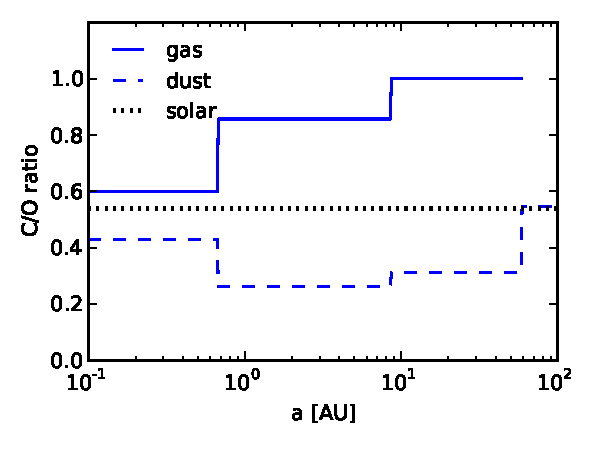
\includegraphics[width=0.8\textwidth]{../figs/C_O_ratio_2.pdf}
%\vspace{-0.5in}
\caption{C/O ratio in gas and in dust as a function of distance, for a passive protoplanetary disk. After \citet{oberg11}.} %  (See text for a description of evolution to yet higher masses.) 
\label{fig:CtoO}
\end{figure}



In addition to the distribution of volatiles in protoplanetary disks, the compositions of planetary atmospheres are also affected by dynamical processes occurring in the disk. For example, solids are redistributed throughout the protoplanetary disk due to radial drift \citep{chiang10}. Observations have shown that young Sun-like stars actively accrete gas from the disk (e.g., \citealt{hartmann06}), which may further change the abundance of volatiles in solid and gaseous form in the disk. 

The chemical composition and the C/O ratio in planetary atmospheres may also change in the late stages of planet formation, as well as due to planetary dynamics. Evaporating planetesimals may pollute the gaseous envelope during runaway atmospheric accretion and late stage accretion \citep{oberg11}. Other dynamical processes such as planetary migration \citep{armitage10} and core dredging (e.g., \citealt{lodders09}) may further affect the atmospheric composition of young planets.

We can thus see that chemical and dynamical processes in protoplanetary disks are tightly connected and highly affect the composition of nascent planets. Exploring and quantifying the effect of all such processes is therefore crucial for our understanding of the formation of giant planets and their overall evolution in the protoplanetary disk. 

\section{Previous Research}

For the past three years I worked on a different project related to planet formation, supervised by Prof. Ruth Murray-Clay and Dr. Andrew Youdin. The goal of my project was to determine the minimum (critical) core mass for a giant planet to form before the gas in the protoplanetary disk dissipates, across a range of semimajor axes between 5-100 AU. This critical core mass is typically quoted to be $\sim$$10$ $M_{\oplus}$. Several previous studies assume steady-state atmospheres heated by planetesimal accretion (e.g., \citealt{stevenson82}, \citealt{rafikov06}). In my work, I chose a complementary approach, in which planetesimal accretion is minimal and the gaseous envelope accretes gas while undergoing Kelvin-Helmholtz contraction. Within this framework, I calculated the critical core mass as a function of disk properties and stellocentric separation. I first assumed an ideal gas polytropic equation of state (EOS) for the nebular gas and an interstellar grain opacity \citep{piso14}. In the followup paper, \citet{piso15}, I used realistic EOS tables to calculate the critical core mass, and explored the effects of a realistic EOS and grain growth opacities on the minimum critical core mass. My results show that the critical core mass for giant planet formation is likely to be lower than 10 $M_{\oplus}$, and steadily decreases with stellocentric distance.

This project has provided me with valuable insights into the process of giant planet formation and has given me the opportunity to extensively review the existing literature on this topic. I believe that the knowledge and experience that I have gained from this project have laid a solid foundation for my current research endeavors in my Ph.D. thesis.

%and planetary migration \citep{armitage10}

\section{Proposed Research}

In this thesis, I plan to investigate the various chemical and dynamical processes that take place in protoplanetary disks, and understand which of these processes are relevant for the chemical variations in the atmospheres of gas giants, and under which conditions. I aim to enhance the toy model of \citet{oberg11} by including dynamical effects, as well as a more complex chemical reaction network. The physical processes that I will consider, as well as the timeline of my thesis, can be summarized as follows. 

\subsection{Radial Drift of Solids and Snowlines Location}
\label{sec:drift}

Solid particles in disks orbit their host star at a Keplerian velocity. The gas, on the other hand, experiences an extra pressure gradient, which causes it to rotate at a sub-Keplerian velocity. Thus dust grains experience a headwind, which tends to remove angular momentum and cause the solids to spiral inwards and fall into the host star. Small grains are well-coupled to the gas, so they rotate with the gas at the sub-Keplerian frequency and their drift timescales are very large compared to the lifetime of the gas disk. Conversely, large planetesimals are decoupled from the gas, thus the influence of gas drag on them is negligible and their radial drift times also exceed the disk lifetime. On the other hand, planetesimals of intermediate sizes ($\sim$0.1cm - $\sim$10 km, depending on their location and the disk temperature and surface density profile) can have short drift timescales relative to the disk lifetime. If  the drift timescale is shorter than the evaporation timescale, solids might drift a significant distance past where a given snowline would be in a passive disk before they desorb. This therefore changes the location and shape of snowlines, and thus the C/O ratio from the profile depicted in Figure \ref{fig:CtoO}.

The calculation of \citet{oberg11} assumes a passive disk. However, observations have shown that young Sun-like stars actively accrete gas from the disk at typical rates $\dot{M}_{\rm gas} \sim 10^{-8}$ $M_{\odot}$/year (e.g., \citealt{hartmann06}). The abundance of H$_2$O, CO$_2$ and CO in gas and grains, and therefore the C/O ratio in gas, will depend on the relative mass accretion rates of solids (due to drift) and of gas (due to viscosity). The surface density of planetesimals (and thus the C/O ratio) is further affected by grain growth and particle fragmentation (e.g., \citealt{birnstiel12}).

I will incorporate the effect of radial drift, particle growth and gas accretion, coupled with the desorption of ices, to calculate the C/O variation with semimajor axis in an actively accreting protoplanetary disk.
\textbf{This will result in Paper I, estimated completion spring 2015}. In this part of my thesis, I will closely collaborate with Dr. Til Birnstiel and use some of his models for grain growth and particle drift as a starting point for my calculations. I also plan to discuss the theoretical aspects of this subproject with Prof. Ruth Murray-Clay.

\subsubsection{Nitrogen Abundance}
\label{sec:nitrogen}

Besides carbon and oxygen, nitrogen is another important volatile molecule that shapes the chemistry in protoplanetary disks. Nitrogen is primarily found as $\rm{N}_2$, although $\sim$$10$\% of the disk nitrogen abundance can be carried by $\rm{NH}_3$ (e.g., \citealt{lahuis00}). I plan to add nitrogen to the simple chemical model of section \ref{sec:drift} and apply the model summarized in section \ref{sec:drift} to study the effect of radial drift on the N/O ratio in protoplanetary disks. Since the main carries of nitrogen in disks are less well understood than those of carbon or oxygen, I will use abundance patterns both from the Solar system and from disk chemistry models (e.g., \citealt{schwarz14}) to define the range of abundances of different carries, then apply the dynamic framework developed in section \ref{sec:drift}. \textbf{This will result in Paper II, estimated completion summer 2015} .

\subsection{The Effect of Time-Dependent Disk Chemistry on the Shape and Location of Snowlines}
\label{sec:chemical}

The calculations summarized in sections \ref{sec:drift} and \ref{sec:nitrogen} are based on a simplified, static chemical model. In reality, however, the gas-grain chemical network in protoplanetary disks is complex and evolves with time (e.g., \citealt{bergin09}, \citealt{fogel11}). Comprehensive disk chemistry models have been developed by several groups, taking into account different radiation fields, dust grain sizes, disk viscosity, time-dependence and dynamics (see references in Table 3 of \citealt{henning13}). These studies have shown that disk chemistry is mostly regulated by disk temperature, density, stellar / interstellar radiation fields, and cosmic rays. Early chemical models of the Solar system were usually restricted to the inner disk regions (10-30 AU) and assumed thermodynamic equilibrium (e.g., \citealt{cameron95}). Due to the decrease in temperature with stellocentric distance, in more modern studies the disk chemistry is divided between the inner disk, $\lesssim$20 AU, and the outer disk beyond 20 AU \citep{henning13}. Due to the absence of intense sources of ionizing radiation, the chemistry in the inner disk approaches quasiequilibrium (e.g., \citealt{ilgner04}). In contrast, high-energy radiation and cosmic rays are key drivers of the chemistry in the outer disk (e.g., \citealt{vandishoeck}), and thus the chemistry is no longer in equilibrium. 

Chemical models of protoplanetary disks are based on detailed chemical kinetics models with hundreds or thousands of chemical reactions, which make them very intensive computationally. These models are thus usually decoupled from disk dynamics. Some studies include various heating and cooling processes, as well as grain evolution (e.g., \citealt{aikawa06}, \citealt{fogel11}, \citealt{vasyunin11}, \citealt{akimkin13}). Additionally, some chemo-dynamical models for protoplanetary disks have been developed --- for example, taking into account radial advective mass transport (e.g., \citealt{aikawa99}, \citealt{woods09}). \citet{semenov11} developed a 2D model using the mixing-length approximation and time-dependent chemistry, for a turbulent disk. They calculated two important timescales, the physical timescale, $t_{\rm phys}$, and the chemical timescale, $t_{\rm chem}$, and found that the chemical evolution is sensitive to changes in the physical conditions if $t_{\rm phys}<t_{\rm chem}$. 

It is thus clear that the chemical processes that occur in protoplanetary disks are very complex, and their coupling with disk dynamics is not always straightforward. I therefore plan to divide this part of my thesis in two steps. First, I will parametrize the detailed, time-dependent chemical reaction network developed by Merchantz et al. (in prep.) and use it in the radial drift calculation described in section \ref{sec:drift}. \textbf{This will result in Paper III, estimated completion fall 2015}. In the second step, I will self-consistently evolve the chemical model from Paper III and the disk dynamics. In order to couple chemistry and dynamics, I will use the tools currently being developed by Xu, Bai \& \"Oberg (in prep.) to reduce the chemical network. I will furthermore  collaborate closely with Ilse Cleeves, who is an expert in chemical evolution in protoplanetary disks. \textbf{This will result in Paper IV, estimated completion spring 2016}. %For this section of my thesis, I will collaborate closely with Ilse Cleeves, who is an expert in chemical evolution in protoplanetary disks.


%In this part of my thesis, I plan to incorporate the detailed, time-dependent chemical reaction network developed by Merchantz et al. (in prep.) \textbf{(?)} in the radial drift calculation described in section \ref{sec:drift}. \textbf{This will result in Paper III, estimated completion late 2015 / early 2016} \textit{(Too much content for one paper? Should it be split into (Paper III) just the effect of evolving disk chemistry on snowline location, and (Paper IV) chemistry + drift?)}.

\subsection{Dynamical Effects II: Core Accretion, Migration, Core Dredging}

The calculations summarized in sections \ref{sec:drift} and \ref{sec:chemical} are focused on the relation between disk chemistry, gas and grain abundances, and disk dynamics. In this part of my thesis, I plan to understand how these disk chemical abundances translate into planetary abundances when taking into account different dynamic effects on defining the disk and the planet formation process. Specifically, I will incorporate dynamic effects such as atmospheric pollution of planetesimals during the atmospheric accretion phase, Type I and Type II migration, and core dredging (e.g., \citealt{lodders09}, \citealt{stevenson85}, \citealt{guillot04}). \textbf{This will result in Paper V, estimated completion summer 2016}. In this part of my thesis I will collaborate closely with Prof. Ruth Murray-Clay.

\subsection{Potential Planet Formation Locations} %and Comparison with Observations}

In the last part of my thesis, I plan to analyze the results obtained in the previous sections, asses the relevance of each chemical or dynamical effect considered, and combine the relevant processes to obtain a realistic framework for analyzing the relation between atmospheric chemical composition and  formation history for a given planet. I will then use this framework to explore a wide parameter space of initial disk conditions in order to generate model planet populations and explore potential planet formation locations. \textbf{This will result in Paper VI, estimated completion spring 2017.}

\section{Auxiliary Projects}

While most of my thesis is focused on theoretical work, I aim to also partake in some observational side-projects. I plan to compare the results of Paper VI with with present and future observations of atmospheric spectra of giant planets, which will be instrumental in constraining their formation, accretion and migration history. For this project, I plan to collaborate closely with the Disk and Astrochemistry groups here at the CfA. 

%By comparing my results with present and future observations of atmospheric spectra of giant planets, I will be able to further constrain their formation, accretion and migration history. \textbf{This will result in Paper V, estimated completion spring 2017.}

\section{Preliminary Results}

As a first step, I investigate the effect of radial drift on the shape of snowlines in protoplanetary disks (see section \ref{sec:drift}). I calculate self-consistently the drift and desorption distances as a function of particle size for a passive disk. I calculate the desorption rates following the prescription of \citet{hollenbach09}, assuming that the solids are perfect spheres and composed of a single volatile material (either H$_2$O, CO$_2$ or CO). To calculate the drift timescale, I follow the analytic prescription of \citet{chiang10}. I integrate the drift and desorption equations self-consistently, and stop the evolution at $\tau=3$ Myr, the typical lifetime of a protoplanetary disk. 

\begin{figure}[htb]
\centering
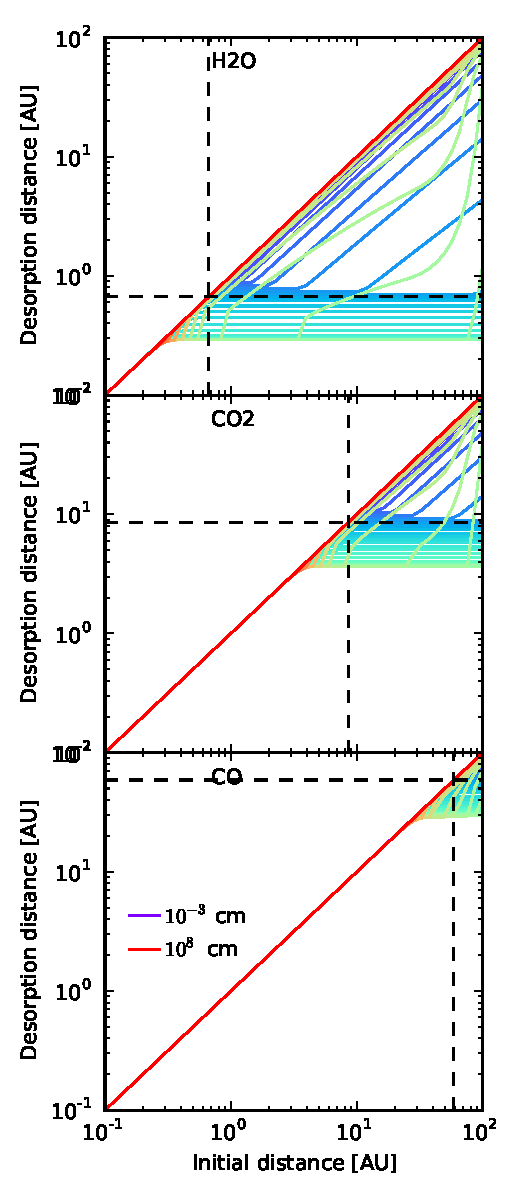
\includegraphics[width=0.47\textwidth]{../figs/desorption_distance_many_new_2.pdf}
%\vspace{-0.5in}
\caption{Desorption distance as a function on initial particle distance for H$_2$O (top panel), CO$_2$ (middle panel) and CO (bottom panel), for particle size between $10^{-3}$ and $10^8$ cm. The vertical and horizontal dashed lines show the respective snowlines as calculated based on \citet{hollenbach09}. Small particles desorb instantaneously, while large particles do not either drift or desorb before disk dissipation. Intermediate size planetesimals desorb at a fixed distance that depends on the particle size, regardless of their initial location in the disk.} %  (See text for a description of evolution to yet higher masses.) 
\label{fig:drift_dist}
\end{figure}

\begin{figure}[htb]
\centering
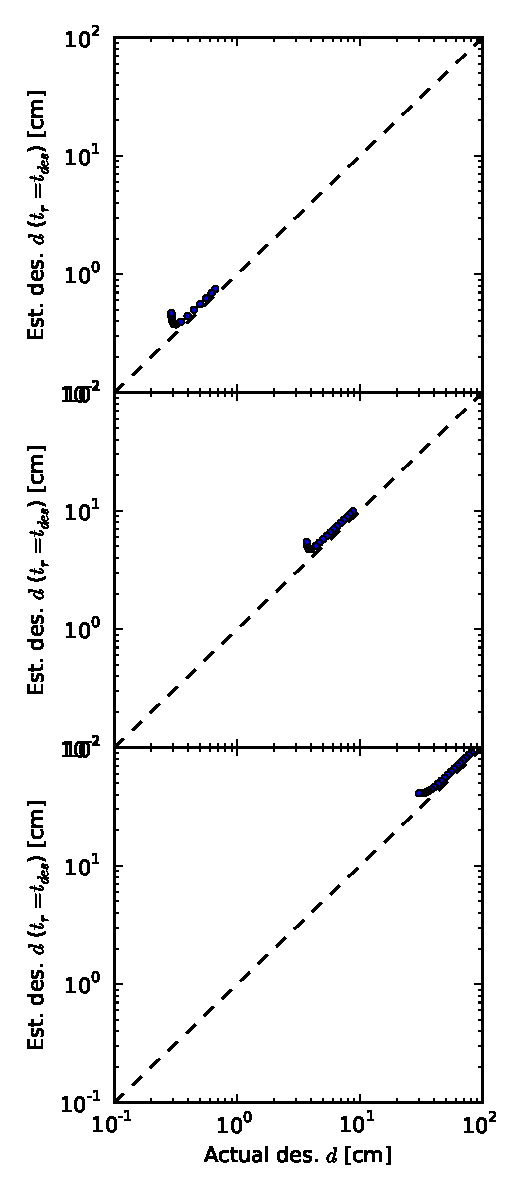
\includegraphics[width=0.5\textwidth]{../figs/desorption_distance_actual_vs_estimated.pdf}
%\vspace{-0.5in}
\caption{Desorption distance estimated analytically (when the drift and desorption times are equal) versus the desorption distance calculated numerically, for H$_2$O (top panel), CO$_2$ (middle panel) and CO (bottom panel), and for different initial particle sizes. The analytic and numerical results are in good agreement.} %  (See text for a description of evolution to yet higher masses.) 
\label{fig:an_vs_num}
\end{figure}

Figure \ref{fig:drift_dist} shows the desorption distance as a function of the initial planetesimal location, for H$_2$O, CO$_2$ and CO particles. As expected, small planetesimals desorb instantly, while large boulders do not have enough time to either desorb or drift before the disk dissipates. Notice, however, that planetesimals with sizes between $\sim 1$ cm and $\sim 10^3$ cm desorb at a fixed distance from the host star, regardless of their initial location in the disk. This desorption distance depends on the planetesimal size. I have found that this distance can be well approximated analytically as the radius at which the desorption and drift timescales are equal (see Figure \ref{fig:an_vs_num}). %Figure \ref{fig:nwater_drift} shows the abundance of H$_2$O with respect to Hydrogen as a function of semimajor axis. We see that particles evaporate most of their mass at their desorption distance (see Figure \ref{fig:drift_dist}). 

\section{Timeline}

\begin{enumerate}
\item Paper I: ApJ, estimated completion Spring 2015.
\item Paper II: ApJ letter, estimated completion Summer 2015.
\item Paper III: ApJ, estimated completion Fall 2015.
\item Paper IV: ApJ, estimated completion Spring 2016.
\item Paper V: ApJ letter, estimated completion Summer 2016.
\item Paper VI: ApJ, estimated completion Spring 2017.
\item Collaborative observational project papers: co-author, estimated completion Summer 2017+
\end{enumerate}


\bibliographystyle{apj}
\bibliography{refs}

\end{document}
